% =====================================================================
% TmFeO3 2DCS — Supplemental Material
% Condensed from tmfeo3_foundation.tex (full derivations there)
% =====================================================================
\documentclass[11pt]{article}
\usepackage{amsmath,amssymb,mathtools,bm}
\usepackage{graphicx}
\usepackage{geometry}
\geometry{margin=2.4cm}
\usepackage{booktabs,array}
\usepackage{xcolor}
\usepackage{hyperref}
\hypersetup{colorlinks=true,linkcolor=blue,citecolor=blue,urlcolor=blue}
\usepackage{cleveref}

\newcommand{\Fe}{\mathrm{Fe}}
\newcommand{\Tm}{\mathrm{Tm}}
\newcommand{\diag}{\mathrm{diag}}
\newcommand{\ket}[1]{|#1\rangle}
\newcommand{\bra}[1]{\langle #1|}
\newcommand{\ve}[1]{\boldsymbol{#1}}
\newcommand{\qafm}{q_{\rm AFM}}
\newcommand{\qfm}{q_{\rm FM}}
\newcommand{\Mnl}{M_{\rm NL}}
\renewcommand{\thesection}{S\arabic{section}}
\renewcommand{\thetable}{S\arabic{table}}
\renewcommand{\thefigure}{S\arabic{figure}}

\title{Supplemental Material for\\
``Reading a magnet's Hamiltonian term by term: two-dimensional terahertz
spectroscopy as vertex spectroscopy of TmFeO$_3$''}
\author{}
\date{\today}

\begin{document}
\maketitle
\tableofcontents

% =====================================================================
\section{The SU(3) qutrit and why its classical dynamics is quantum-exact}
\label{si:qutrit}
% =====================================================================

Tm$^{3+}$ is $4f^{12}$, $^3H_6$ ($J=6$).  In the $C_s(m)$ crystal field of
the $Pbnm$ $4c$ site the 13-fold multiplet splits into 13 singlets; the
model keeps the three lowest, $\ket{1},\ket{2},\ket{3}$, with splittings
$E_{12}=2.068$\,meV ($0.50$\,THz) and $E_{13}=4.963$\,meV ($1.20$\,THz),
consistent with the measured lines $E_{12}+E_{23}\approx E_{13}$.  The
site state is the Gell-Mann vector $\lambda^a=\mathrm{Tr}(\rho\Lambda^a)$,
$a=1\dots8$, and every single-ion term (CEF energies, external drives,
exchange mean fields) is \emph{linear} in the $\Lambda^a$.  For a
Hamiltonian linear in the generators the von Neumann equation
$\dot\rho=-i[H,\rho]$ closes on $\vec\lambda$:
\begin{equation}
  \dot\lambda^a \;=\; \Omega_{ab}(t)\,\lambda^b
  -\gamma_a\big(\lambda^a-\lambda^a_{\rm eq}\big),\qquad
  \Omega_{ab}=\tfrac12\,\mathrm{Tr}\!\left(\Lambda^a\,
  (-i)[H(t),\Lambda^b]\right).
\end{equation}
The classical SU(3) propagation is therefore the \emph{exact} quantum
dynamics of the driven, damped three-level ion, and a Boltzmann-weighted
ensemble of trajectories launched from the level seeds
$\ket1,\ket2,\ket3$ is the exact thermal density matrix for single-ion
drives.  (This was verified explicitly against an independent
density-matrix integrator; the two censuses agree to all digits quoted.)
Damping is Bloch-type on the Gell-Mann pairs of each transition,
$\gamma(\lambda^{1,2}),\gamma(\lambda^{4,5}),\gamma(\lambda^{6,7})$, with
population relaxation $\gamma(\lambda^{3,8})$ toward the equilibrium
populations captured at initialization.

The magnetically bright coordinate of the $E_{12}$ block follows from the
projected moment $P J_z P=5.264\,\lambda^2$: only $\lambda^2$ radiates
magnetically, and the onsite splitting drives the planar precession
$\dot\lambda^1=-\Delta_{12}\lambda^2$,
$\dot\lambda^2=+\Delta_{12}\lambda^1$, so the $E_{12}$ sector is a single
driven oscillator
\begin{equation}
  \lambda^2(t)=\int_0^t \sin[\omega_{12}(t-t')]\,h^1(t')\,dt',
  \label{eq:si-osc}
\end{equation}
where $h^1$ is the effective force a conversion vertex exerts on
$\lambda^1$.  All delay-axis structure of a cross peak lives in the
$\tau$-dependence of $h^1$.

% =====================================================================
\section{Crystallography and the projected Fe--Tm coupling}
\label{si:crystal}
% =====================================================================

TmFeO$_3$ is $Pbnm$ ($Z=4$): Fe$^{3+}$ at $4b$ (site symmetry $\bar1$;
every Fe sits on an inversion center), Tm$^{3+}$ at $4c$ (site symmetry
the single mirror $m_z$).  Inversion maps each Fe sublattice to itself
and exchanges Tm sublattices in pairs; the local mirror is the physical
$4c$ site mirror and generates the relative $\lambda^5,\lambda^7$ signs
between Tm sublattices.  The Fe order is G-type
($T_N\approx632$\,K) with DM canting; below the spin reorientation
($T_2\approx85$\,K) the ground state is $\Gamma_2=(F_x,C_y,G_z)$.

The Fe--Tm sector is built from the physical operator route
\begin{equation}
  \ve S,\ \ve J\ \longrightarrow\ H_{\Fe-\Tm}=\ve S^TA\,\ve J
  \ \longrightarrow\ P\ve JP
  \ \longrightarrow\ \text{couplings to }\lambda^a ,
\end{equation}
never by assuming that a space-group rotation acts as a closed onsite
SU(3) rotation in one fixed qutrit basis.  Working in a
\emph{transported gauge} (qutrit bases on the four Tm sublattices related
by the group operations themselves) makes every bond formula explicit and
turns the irrep ($\Gamma_1$) projection into simple four-site sign sums.
Time-reversal splits the Gell-Mann set into
$\lambda^-=\{\lambda^2,\lambda^5,\lambda^7\}$ (odd) and
$\lambda^+=\{\lambda^1,\lambda^3,\lambda^4,\lambda^6,\lambda^8\}$ (even);
every coupling term must be $\mathcal T$-even overall, which fixes how
many Fe-spin or $B$-field legs may attach to each sector.  The candidate
couplings through cubic order in the fields are
\begin{center}
\renewcommand{\arraystretch}{1.25}
\begin{tabular}{llll}
\toprule
family & operator form & sector & legs \\
\midrule
$K^-$ & $S_\alpha\lambda^a$ & $\lambda^-$ & 1 Fe \\
$ESJ$ & $E_\eta S_\alpha\lambda^a$ & $\lambda^-$ & 1 E-photon + 1 Fe \\
$\kappa^B$ & $B_\eta S_\alpha\lambda^a$ & $\lambda^+$ & 1 B-photon + 1 Fe \\
$W$ & $S_\alpha S_\beta\lambda^a$ & $\lambda^+$ & 2 Fe \\
\bottomrule
\end{tabular}
\end{center}
The full orbit formulas (all eight coefficients per bond, all four Tm
sublattices, both time-reversal sectors) and the implementation
prescriptions for global-axis versus local-frame storage are given in the
long-form working note that accompanies the data
(\texttt{tmfeo3\_foundation.tex}, Secs.~3--14).

% =====================================================================
\section{The sharp requirement and the vertex scorecard}
\label{si:scorecard}
% =====================================================================

Two collinear pulses give $\Mnl=M_{AB}-M_A-M_B$; order by order only the
mixed terms survive, so $\Mnl$ starts at second order and the leading
robust magnetic-dipole contribution is third order.  Combining
Eq.~\eqref{eq:si-osc} with the conservation rules at each vertex (energy;
$\mathcal T$-parity; $\Gamma_1$) yields six requirements for a coupling
to produce the geometry-A cross peak at $(\qafm,E_{12})$:
\begin{description}
\item[R1 (detection)] reaches $\lambda^1/\lambda^2$ (the $E_{12}$ block);
\item[R2 (drive)] is sourced by the pumped $\delta S_y$ magnon;
\item[R3 (parity)] is $\mathcal T$-even (fixes the $\lambda^\pm$ sector);
\item[R4 (irrep)] is $\Gamma_1$-allowed in the $\Gamma_2$ state;
\item[R5 (energy)] carries the $0.90\to0.50$\,THz mismatch (needs $\geq2$
  non-$\lambda$ legs);
\item[R6 ($\Mnl$)] involves both pulses.
\end{description}

\begin{table}[h]
\centering\small
\caption{Vertex scorecard.  Only $W$ and $\kappa^B$ pass all six
requirements; the final model uses the static $W$ family alone, the
geometry-B transfer being fed by the electric quadrature of the drive
rather than by a field-assisted vertex.}
\begin{tabular}{lccccl}
\toprule
vertex & legs & sector & R1 & R2--R6 & verdict\\
\midrule
$K^-$ & $1\Fe+1\Tm^-$ & $\lambda^-$ & $\times$ & $\times$ &
  hybridizes only; $\Gamma_1$-blocked; reorients $\Gamma_2$\\
$ESJ$ & $E+\Fe+\Tm^-$ & $\lambda^-$ & $\times$ & \checkmark &
  real, but feeds $E_{13}/E_{23}$, not $E_{12}$\\
$W$ & $2\Fe+\Tm^+$ & $\lambda^+$ & \checkmark & \checkmark &
  \textbf{winner}: rank-1, factorized peak\\
$\kappa^B$ & $B+\Fe+\Tm^+$ & $\lambda^+$ & \checkmark & \checkmark &
  passes, but superseded (not in the final model)\\
\bottomrule
\end{tabular}
\end{table}

\paragraph{$K^-$ fails threefold.}
(i) Linear in $S$, it only rotates the harmonic normal-mode basis:
coupled harmonic oscillators give diagonal peaks only; a static bilinear
conserves energy and cannot convert $0.90$ into $0.50$\,THz.
(ii) The $\Gamma_1$ orbit sums vanish for every channel except
$K^-_{2y}$: a static one-at-a-time scan at $0.2$\,meV leaves the energy,
the Fe order, and the uniform $(\lambda^2,\lambda^5,\lambda^7)$
\emph{bit-identical} to baseline for all components except $2y$.
(iii) The one allowed channel $K^-_{2y}$ is a transverse molecular field
on the order parameter and reorients $\Gamma_2\to G_y$ between $0.085$
and $0.090$\,meV---it is not a perturbative vertex.  Full-dynamics 2DCS
on the inert channels ($K^-_{2x}$ up to $1.5$\,meV, $K^-_{2z}$ up to
$2.0$\,meV) leaves the induced $\lambda^2$ at machine precision
($\leq7\times10^{-15}$).

\paragraph{The two winners.}
The two-magnon vertex rectifies the pulse-A/pulse-B cross term,
\begin{equation}
  h^1_{\rm NL}(t,\tau)=W^{yy}_1A^2\left[\cos(\qafm\tau)
  -\cos(\qafm(2t+\tau))\right]\theta(t)
  \;\Rightarrow\;
  \Mnl^{W}\propto\cos(\qafm\tau)\,[1-\cos\omega_{12}t],
\end{equation}
a clean factorized peak with no diagonal partner.  The field-gated
vertex kicks at the probe, $h^1\propto B_y(t)S_y(t)$ with
$S_y(0)=A\sin\qafm\tau$, giving
$\Mnl^{\kappa}\propto\sin(\qafm\tau)[1-\cos\omega_{12}t]$: also on
target.  It is, however, not required.  The one physical geometry-B
pulse carries an electric quadrature, $E\!\parallel\!a$ acting through
$d_x\lambda^1$, which writes the $E_{12}$ coherence directly; the
static $W^{xz}_1$ at its master value then converts the stored
coherence into the magnon, and the measured transfer peak is
reproduced with $\kappa^B=0$.  The polarisation ownership of $d_x$
supplies the geometry selection the $B_z$ gate supplied before: the
component does not exist in geometry A.

\paragraph{Exhaustion of the quadratic families.}
All remaining symmetry-allowed quadratic couplings were switched on one
at a time in the full nonlinear dynamics and are exactly inert
(differences at the $10^{-12}$ level or below): $W_4^{yy,xy,yz,xx,zz,xz}$,
$W_1^{xy}$, $W_6^{yy,xz}$, $\kappa^E_{2y}$, $\kappa^E_{5x}$.  Among the
$W_1$ components: $W_1^{yz}$ couples the qutrit to the $A_y/C_y$
exchange modes (wrong magnon irrep---verified by the upper-branch ghost
row at $1.4$\,THz under strong coupling), $W_1^{zz}$ negligible,
$W_1^{xx}$ alive but floods the spectrum with an $\omega_t=0.16$\,THz
comb, and $W_1^{xz}$ is the on-target converter.  No static component
converts a \emph{magnetically} written coherence without entering the
mixer regime (level repulsion dragging the $E_{12}$ line, excluded by
1D absorption at every strength---verified with the bare splitting
recalibrated at each coupling so the dressed line stays at its measured
position, which preserves $E_{12}{+}E_{23}{=}E_{13}$ automatically).
The \emph{electrically} written coherence requires no such regime: the
master $W^{xz}_1=0.01$ suffices, and the field-assisted family is
retired by parsimony rather than by symmetry.

% =====================================================================
\section{Numerical protocol}
\label{si:numerics}
% =====================================================================

\paragraph{Dynamics.}  Classical LLG for Fe (unit spins, $S=5/2$ scale
absorbed), SU(3) Bloch dynamics for the four Tm sublattices; RK4 with
$\Delta t=0.02$ code units; $1\times1\times1$ cell of the $Pbnm$
magnetic unit (8 Fe + 4 Tm).  Time is measured in $\hbar/$meV; a
frequency $f$ in THz corresponds to $E=f\times4.136$\,meV.

\paragraph{2DCS protocol.}  Delay scan $\tau\in[-120,0]$ code units,
$\Delta\tau=0.1$ ($0.2$ for scans); detection window to
$t_{\max}=160$ for $0.01$\,THz resolution on $\omega_t$.  The nonlinear
signal is the honest three-run subtraction
$\Mnl=M_{AB}-M_A-M_B$ per delay; no pulse-window chunking; no reuse of
the reference run across delays (both shortcuts were found to
contaminate spectra and are documented pitfalls).  The pump enters as a
tabulated waveform (the measured field, times converted
$t_{\rm code}=t_{\rm ps}/0.6582$, auto-centered and normalized).

\paragraph{Spectra and blind peak census.}  2D spectra are
$|\mathrm{FFT}_{\tau,t}|$ of $\Mnl$ with a detection window $t\geq3$
(excludes pulse overlap).  Cross-polarised channels use Hann windows on
both axes; the same-polarised channel uses its documented convention, a
cosine gate over the pulse-overlap region of the delay axis
($|\tau|<6$ code units) with Gaussian $t$-apodization to $0.03$.
Spectra are lightly smoothed ($1\times0.5$ pixels) and displayed on a
linear amplitude scale.  The delay axis is
plotted physically ($\omega_T=-\omega_\tau^{\rm FFT}$;
$+$\,=\,non-rephasing).  Peaks are accepted only by a blind census:
2D local maxima (maximum filter, $0.10$\,THz neighborhood) with
prominence $\geq1.5$ over the local median background
($0.34$\,THz annulus) and amplitude $\geq5\%$ of the map maximum,
merged within $0.09$\,THz.  Rectified ($\omega_t\approx0$) content is
analyzed separately via $S_{\rm DC}(\tau)=\langle\Mnl\rangle_t$ with
cubic drift removal.  The $\omega_\tau=0$ pump--probe row is retained
in the displayed geometry-A panels, as in the measured maps, auto-scaled
to the measured relative row amplitude (the raw row is dominated by
broadband pump--probe drift; the applied factor is recorded in the
census file); rows with $|\omega_\tau|<0.18$\,THz are excluded from
all censuses, since they carry pump--probe rather than delay-coherence
information.  Radiation bookkeeping used throughout: for
$k\parallel b$, M1 dipoles radiate $E\propto\hat k\times m$, so the
$E\parallel c$-detected channel carries $d_z(\lambda^2)+m_x$ and the
$E\parallel a$-detected channel carries $d_x(\lambda^{5,7})+m_z$.

\paragraph{Thermal ensembles.}  Boltzmann mixtures of trajectories from
the level seeds $\ket1,\ket2,\ket3$ (Sec.~\ref{si:qutrit}).  Two
documented pitfalls: (i) any pre-dynamics energy minimization collapses
excited-level seeds and must be disabled; (ii) population damping
$\gamma(\lambda^{3,8})$ relaxes toward the equilibrium captured at
initialization, which must therefore be captured per-seed.

% =====================================================================
\section{Experimental inputs}
\label{si:exp}
% =====================================================================

\begin{table}[h]
\centering\small
\caption{Measured mode parameters and the derived simulation inputs.
CEF damping is Bloch on the Gell-Mann pair of each transition,
$\gamma_a[\mathrm{meV}]=\gamma[\mathrm{THz}]\times h$; magnon damping is
Gilbert, $\alpha=\gamma/2\nu$ fixed by the $\qafm$ line.  Emission
weight is $\sqrt f$ (E1) for the CEF lines and M1 for the magnons.
The last column is the measured pulse spectral amplitude at each mode.}
\begin{tabular}{lcccccl}
\toprule
mode & $\nu$ [THz] & $f$ & $\sqrt f$ & $\gamma$ [THz] & damping (sim) &
pulse amp.\\
\midrule
$\qfm$  & 0.38 & 0.08 & 0.28 & 0.005 & $\alpha=1.7\times10^{-3}$ & 0.92\\
$\qafm$ & 0.90 & $7\times10^{-4}$ & 0.026 & 0.003 & $\alpha=1.7\times10^{-3}$ & 0.68\\
$E_{12}$ & 0.50 & 6.5 & 2.55 & 0.038 & $\gamma(\lambda^{1,2})=0.157$\,meV & 1.00\\
$E_{23}$ & 0.70 & 6.6 & 2.57 & 0.10  & $\gamma(\lambda^{6,7})=0.414$\,meV & 0.85\\
$E_{13}$ & 1.20 & 8.7 & 2.95 & 0.05  & $\gamma(\lambda^{4,5})=0.207$\,meV & 0.36\\
\bottomrule
\end{tabular}
\label{tab:si-exp}
\end{table}

\begin{figure}[h]
\centering
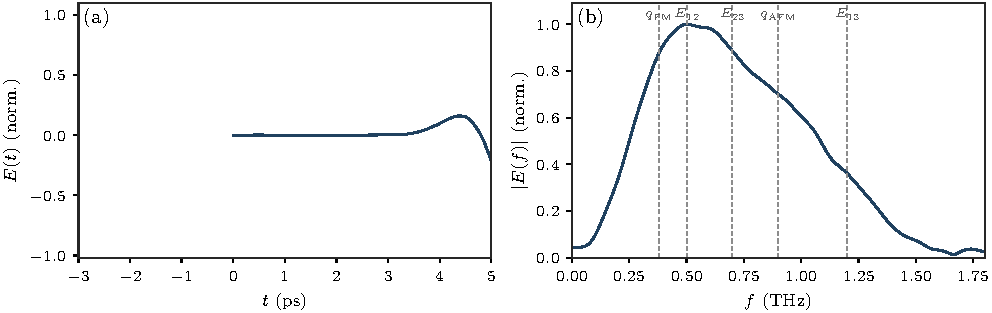
\includegraphics[width=0.95\textwidth]{figs/experimental_pulse_final.pdf}
\caption{The measured THz pump.  Left: single bipolar cycle
($\sim1.2$\,ps, no DC).  Right: amplitude spectrum peaked at
$0.50$\,THz$\,=E_{12}$, covering all five modes.  The smallness of
DC content removes the quasistatic-tilt legs that a Gaussian stand-in
pulse would add; the measured waveform is the cleanest configuration.}
\label{fig:si-pulse}
\end{figure}

Two consequences organize the readout physics.  First, excitation
scales as $E^2$ and detection as $E^1$ (third order).  Second, the CEF
lines are E1-bright while $\qafm$ is E1-dark but M1-bright: a magnon is
therefore read out either by borrowing a CEF electric dipole through an
Fe--Tm vertex (geometry A) or through its own magnetic dipole at the
magnon frequency (geometry B).  Using the magnetic $g$-factor instead of
$\sqrt f$ for the magnon electric emission over-weights it by
$\sim100\times$ and buries the CEF peaks under the magnon diagonal; the
oscillator-strength weighting resolves this without any tuning.

% =====================================================================
\section{Displacive verification of the $W$ mechanism}
\label{si:displacive}
% =====================================================================

The rectified two-magnon force is a suddenly switched step: its edge
carries spectral weight $\propto e^{-\omega_{12}^2\sigma^2/2}$ at the
CEF frequency, i.e.\ the $E_{12}$ quantum is drawn from the pulse
bandwidth (intra-pulse difference-frequency/impulsive-Raman), while the
magnon pair carries only the phase memory $\cos\qafm\tau$.  Verified
directly: stretching the pulse $\sigma=0.25\to1.0$ at fixed amplitude
collapses the peak by $4.5$ decades ($51.7\to1.7\times10^{-3}$), while
switching the direct Tm drive on/off changes it by $<10^{-4}$
(pure-$W$ origin).  The same sweep resolves the second Fe leg: impulsive
pulses use the resonant probe magnon (peak $\propto A^2$); longer pulses
cross over to the field-following quasistatic tilt (peak
$\propto A^1$).  The measured no-DC waveform suppresses the quasistatic
legs, which is why the experimental pulse yields the cleanest spectra.

% =====================================================================

% =====================================================================
\section{Geometry B: the transfer and the post-drive buildup}
\label{si:buildup}
% =====================================================================

\begin{figure}[h]
\centering
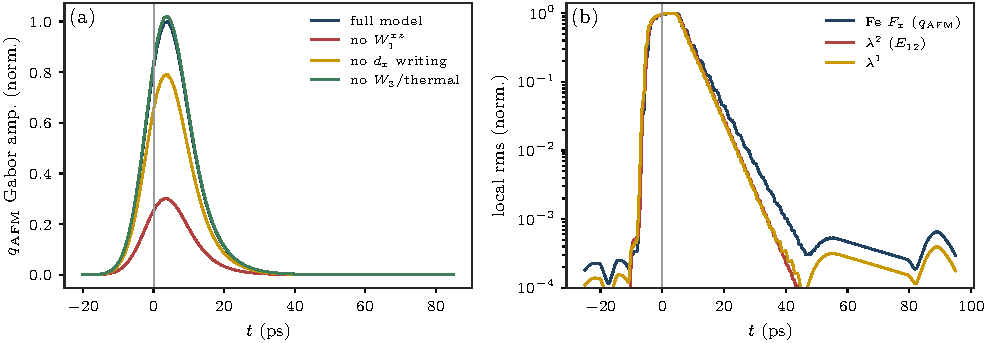
\includegraphics[width=0.95\textwidth]{figs/postdrive_buildup_final.pdf}
\caption{No coherence-fed post-pulse buildup once the measured
linewidths are enforced (single measured pulse, geometry B; Gabor
amplitude at $0.90$\,THz, $\sigma=5$\,ps).  (a)~The $\qafm$ amplitude
peaks \emph{at} pulse end and decays with
$\tau_{\rm env}\approx8$\,ps $=T_2(E_{12})$ in the full model and in
every term ablation; the terms set the absolute scale (removing
$W^{xz}_1$ or the $d_x$ writing lowers the peak, removing
$W_3$/thermal changes nothing) but none produces post-pulse growth.
(b)~All coherent reservoirs die within their measured $T_2$ (log
scale); the weak late-time floor is the incoherent thermal tail,
orders of magnitude below the impulsive peak.}
\label{fig:si-buildup}
\end{figure}

The geometry-B cross channel is analysed on the Fe $m_x$ dipole with
its Tm part identically zero (subalgebra closure), so it reads the
magnon amplitude directly.  Its transfer peak $(E_{12},\qafm)$ is the
energy face read backward: a stored $1\!\leftrightarrow\!2$ coherence
handed to the quasi-antiferromagnetic magnon.  Isolated-drive runs
settle the anatomy.  With the coherence written \emph{magnetically}
($\mu_z\lambda^2$ only) at the master $W=0.01$ the conversion is
inefficient and the map fills with drive-squared diagonals; adding the
\emph{electric} quadrature of the same physical pulse
($d_x\lambda^1$, the component only $E\!\parallel\!a$ possesses)
produces the transfer row at the \emph{unshifted} $E_{12}$ position,
at the measured amplitude for $w_{E1}=0.54$, with strays below
$0.17$.  The interference of the two quadratures places the row at
$\omega_\tau=0.52$ for $\mathrm{sign}(d_x\mu_z)<0$, as measured.  The
leave-one-out runs (Sec.~\ref{si:audit}) quantify the shares at the
operating point: removing the electric writing halves the transfer
($0.49$), removing $W^{xz}_1$ costs a quarter ($0.76$), the remainder
flowing through the magnetically written quadrature and the
$W^{yy}_1$ mixing route ($\qfm{+}E_{12}=0.88$, unresolved from
$\qafm$); in every ablation the emission stays pinned at
$0.900$\,THz---all routes ultimately ring the real $\qafm$ mode.  No
field-assisted vertex appears anywhere ($\kappa^B=0$; its inertness in
these geometries is bitwise, Sec.~\ref{si:codeaudit}).

The measured signal, however, continues to grow after the pulse, and
within this coupling space no channel reproduces growth at the peak's
own scale (Fig.~\ref{fig:si-buildup}): every coherent pathway inherits
its source's lifetime, and with $T_2(E_{12})=8$\,ps everything
coherent is over within $\sim10$\,ps.  The one reservoir that outlives
every $T_2$---the CEF populations, fed incoherently by the dissipated
pulse energy and acting on the magnon through the population channel
$W_3$---produces a persistent, drive-uncorrelated tail roughly four
decades below the impulsive peak.  The buildup at the peak's own scale
therefore stands as the one timing observable outside this coupling
space; the same incoherent reservoir is read optically by the
rectified $(\pm E_{12},\omega_t\!\to\!0)$ line of the same-polarised
channel, whose strength relative to $(E_{12},E_{23})$ calibrates
$c_{\rm heat}W_3$.

% =====================================================================
\section{Propagation: self-absorption of the electric-dipole light}
\label{si:propagation}
% =====================================================================

The sample is optically thick at the strong $E1$ crystal-field lines
($f=8.7$ at $E_{13}$, depth $\simeq6$; depth $\simeq1$ at $E_{12}$),
and the same transmission filters the incoming field and the emitted
$E1$ light; magnetic-dipole radiation passes freely.  The filter is
implemented as a Lorentzian optical depth on the $E1$ components,
\begin{equation}
  T(\omega)=\exp\!\Big[-\frac{d}{1+\big((\omega-\omega_{13})/
  \gamma_{13}\big)^{2}}\Big],\qquad d\simeq6,
\end{equation}
applied to the emission column \emph{and} to the delay-axis free
induction decay of any electrically written coherence.  Three measured
structures follow with no further freedom.  (i) The two
$E_{13}$-emission features sit at $\omega_t=1.15$ and $1.25$\,THz, one
absorption linewidth below and above the $1.20$ line: self-reversal
wings of an optically thick line, whose centre is dark
($T\simeq0.002$).  (ii) The two-quantum $(E_{13},E_{23})$ row, which
the free-ion model robustly produces at $0.33$ (the pump reaching
$\rho_{13}$ at second order), is removed \emph{exactly} by the FID
reabsorption on the delay axis---the model value falls to $0.00$ with
the filter, and the measurement contains no $\omega_\tau=E_{13}$
feature.  (iii) The SFG tone of Sec.~\ref{si:sfg} escapes at $1.41$,
one linewidth \emph{outside} the opaque window ($T=0.68$), which is
why it is visible while the line centre is not.  Every wing amplitude
scales with sample thickness: a thin sample revives the $E_{13}$
centre and the two-quantum row \emph{together}, the decisive
propagation test.

% =====================================================================
\section{The same-polarised channel at the final operating point}
\label{si:samepol}
% =====================================================================

The channel is analysed by the minimal
$(E\!\parallel\!c,H\!\parallel\!a)$ operator
\begin{equation}
  O_1=F_x+0.913\,\lambda^7+4.4\,\lambda^6
      +g_d(\langle F_x\rangle+\delta F_x)\lambda^2 ,
\end{equation}
with $\mu^x_{13}=0$ and $d_z(1\!\to\!3)\leq0.006$ (bounded by the weak
$1.15$ wing and dropped), the Fe weight bounded above by the absent
magnon diagonal ($c_{\rm Fe}\to0$; the diagonal sits at $0.13$, below
the digitisation threshold), and the propagation filter of
Sec.~\ref{si:propagation} applied to the $E1$ components.

\emph{The fully dark $1\!\to\!3$ dipole is measured, not assumed.}
The measured map contains delay frequencies
$\omega_\tau\in\{E_{12},\qafm\}$ only; a bright $\mu^z_{13}$ would
store an $E_{13}$ coherence at first order and produce an
$(E_{13},E_{23})$ peak with exactly the dipole product of the observed
$(E_{12},E_{23})$.  The analyser moreover physically contains
$\mu_x\lambda^5$, and at the point-charge value $\mu^x_{13}=2.39$ that
single term would exceed the whole measured map by two orders of
magnitude: $\mu^x_{13}$ fits to zero.  The transition is magnetically
dark in every polarisation; its large measured oscillator strength is
electric and is precisely what makes the sample opaque at
$1.20$\,THz.

\emph{Final accounting.}  With the cross channels held fixed:
\begin{center}\small
\renewcommand{\arraystretch}{1.2}
\begin{tabular}{lccl}
\toprule
peak & experiment & model & mechanism\\
\midrule
$(E_{12},E_{23})$ & $1.00$ & $1.00$ &
  coherence$\to$population$\to\rho_{23}$, non-rephasing\\
$(E_{12},0.40)$ & $0.45$ & $0.40$ & cascade tone
  $2(E_{23}{-}E_{12})$, adjacent to $\qfm=0.38$\\
$(E_{12},0.90)$ & $0.40$ & $0.43$ & cascade tone $2E_{23}{-}E_{12}$,
  degenerate with $\qafm$\\
$(\qafm,E_{12})$ & $0.30$ & $0.39$ & magnon$\to$Tm via
  $d_z^{\rm eff}$ (reciprocity partner)\\
$(\qafm,\qafm)$ & absent & $0.13$ & magnon diagonal; the null bounds
  $c_{\rm Fe}$\\
$(E_{13},E_{23})$ 2Q & $0$ & $0.00$ & killed exactly by FID
  reabsorption\\
$(E_{12},1.15)$ & $0.15$ & $0.02$ & $E_{13}$ wing; bounds
  $d_z(1\!\to\!3)$\\
$(\qafm,1.41)$ & $0.30$ & $0.31$ & SFG tone $\qafm{+}E_{12}$
  (Sec.~\ref{si:sfg})\\
$(\qafm,0.40)$ & obs. & $0.43$ & DFG tone $\qafm{-}E_{12}$\\
$(E_{12},1.41)$ & obs. & $0.36$ & $E_{12}$-delay partner of the SFG\\
$(-E_{12},E_{23})$ & $<0.15$ & $\sim0.7$ & \textbf{open}: residual R1\\
\bottomrule
\end{tabular}
\end{center}

\emph{Cascade tones at the magnon frequencies.}  The two
$E_{12}$-delay features at $0.40$ and $0.90$ survive the
\emph{no-magnon} ablation at $0.89$--$0.97$ and die without the
$\lambda^7$ drive leg ($0.05$--$0.08$): they are intrinsic tones of
the driven three-level cascade, $2(E_{23}{-}E_{12})$ and
$2E_{23}{-}E_{12}$, numerically coincident with $\qfm$ and $\qafm$.
The genuine Tm$\to$magnon transfer is the $\lesssim10\%$
Zeeman-sensitive remainder.  Positionally the low tone sits at
$0.40$, a full linewidth above $\qfm=0.38$---a direct experimental
discriminator---and cascade tones survive the spin reorientation with
CEF width, while magnon sidebands would soften and sharpen.

\emph{Exact single-ion verification.}  A standalone integrator of the
8-dimensional $\vec\lambda$ equation (same CEF energies, dampings,
measured pulse, same census pipeline; $\sim13$\,s per 2D map)
reproduces the lattice $E_{12}$-family census exactly, proving the
family is single-ion physics and enabling exhaustive scans.  Two
facts emerge: the rephasing/non-rephasing ratio of the
$(E_{12},E_{23})$ transfer has a floor of $0.47$--$0.58$ under this
pulse across all drive strengths, dipole phases and dampings---the
\emph{rephasing remnant is an exact property of any three-level ion
driven by this waveform}, and it is the one residual (R1) the model
does not remove, the measured negative-delay side carrying only the
rectified and $\qfm$ features.  The SFG/DFG tones contribute
rephasing partners of their own there (model $0.5$--$0.7$).  This
residual, the wing amplitudes, and the geometry-B $d_z^{\rm eff}$
doublet strength all funnel into one measurable object: the sample's
polarisation-resolved optical depths at the three CEF lines.

% =====================================================================
\section{The dynamical $d_z^{\rm eff}$: internal magnon--CEF SFG and DFG}
\label{si:sfg}
% =====================================================================

The order-induced dipole is the $ESJ$ vertex
$-g_d E_z(F_x\lambda^2)$; condensing its spin leg on
$\langle F_x\rangle$ gives the drive and linear-emission avatars, and
the retained fluctuation $g_d\,\delta F_x\lambda^2$ is a bilinear
emitter radiating at $\qafm\pm E_{12}=1.40/0.40$\,THz with the magnon
on the delay axis.  Because the trajectory pack stores the full time
evolution of every coordinate, any candidate product moment
$X_iX_j$ is evaluable post hoc with no new simulation:
$P_{\rm NL}=X^{AB}_iX^{AB}_j-X^{B}_iX^{B}_j-X^{0}_iX^{0}_j$ per
delay, followed by the standard census.  A sweep of all $33$
symmetry-classified Fe--Fe ($F$/$G$ bilinears) and Fe--Tm
($F/G\times\lambda^{1,2}$) products gives a sharp verdict:
\begin{itemize}
\item Every single-coordinate (linear) channel and all four remaining
  on-site quadratic moments of the $4c$ site
  ($\lambda^1\lambda^6,\lambda^2\lambda^7$ as $d_z$;
  $\lambda^1\lambda^7,\lambda^2\lambda^6$ as $m_x$) radiate at
  $E_{12}{+}E_{23}=1.20$\,THz with an $(E_{12},1.20)$ partner
  $10$--$12\times$ their $\qafm$-row feature---opposite to the
  measured ratio.  The measured smallness of $(E_{12},1.20)$ bounds
  all four at once.
\item The Fe--Fe striction products ($G_xG_y$, $F_yG_y$) land at
  $\qafm{+}\qfm=1.28$ with the right ratio but carry full-strength
  combination delay rows at $|\omega_\tau|=1.05/1.49$ that the
  measurement lacks.
\item $\delta F_x\lambda^2$ (with its $m_x$-type siblings) is the
  \emph{only} channel of the catalogue whose 2D map is led by the
  $\qafm$-delay row (partner ratio $1.4$--$1.6$ instead of the
  universal $\sim0.1$): both of its factors are written at first
  order by the same pulse, so the stored magnon pays no conversion
  penalty.  The term-ablation runs confirm exactly this---the tones
  survive removal of both $W$ components ($0.95$--$1.02$) and die
  only with the Zeeman or electric drive legs.
\end{itemize}
One number is fitted: the condensation-ratio correction $s=0.42$ on
the naive trajectory weight $\delta F_x/\langle F_x\rangle$ (the
model's canting angle, $\langle F_x\rangle=8.4\times10^{-3}$ per
spin, overestimates the ratio by about two).  The sum tone then lands
at the measured $(\qafm,1.41)=0.30$; the difference tone at $0.43$
merges into the measured $(\qafm,E_{12})$ blob; the $E_{12}$-delay
partner appears at $0.36$.  Together with the on-site
$\beta\lambda^1\lambda^2$ these complete the $\chi^{(2)}$-like triad
of the inversion-free rare-earth site in emission---SHG (degenerate),
SFG and DFG (non-degenerate, cross-subsystem)---with the mixing
element a bilinear term of the material's transition moment, not a
crystal-optical $\chi^{(2)}$ acting on light.  The triplet is
over-constrained: locked ratios, position at $\qafm{+}E_{12}$ exactly
(at $1.20$ it would be a quadratic moment, and the dark $E_{13}$
window separates the cases), tracking of the softening magnon, and
collective collapse at the reorientation with everything that rides
$g_d\propto\langle F_x\rangle$.

% =====================================================================
\section{One drive for one experiment: the operating point}
\label{si:operating}
% =====================================================================

The two geometry-A channels are the same measurement---same
$H\!\parallel\!a$, $E\!\parallel\!c$ excitation, differing only in the
detected polarisation---so they share one drive, and the Tm and Fe
drive amplitudes are tied by the $g$-factor ratio:
$A_{\rm Tm}=g_{\rm ratio}|v|A_{\rm Fe}$.  Fluence is therefore the
single drive parameter, and the cross channel measures it.  At strong
drive ($A_{\rm Fe}=1.2$) the channel is nonperturbative: the $E_{12}$
diagonal reaches $1.45$ of the $(\qafm,E_{12})$ peak and a forest of
multi-magnon strays appears at
$\omega_\tau=0.63,0.72,0.99,1.25,1.51$\,THz, none observed.  Lowering
the fluence removes them monotonically (the diagonal falls to $0.56$,
$0.16$, $0.06$ at $A_{\rm Fe}=0.4$, $0.12$, $0.04$), so the experiment
sits in the perturbative regime; the production operating point is
$A_{\rm Fe}=0.12$ (geometry B independently at $0.10$).  The former
second drive dial---a residual $\mu^z_{13}$ admixture---is gone: the
$1\!\to\!3$ transition is fully dark as a \emph{measured} statement
(Sec.~\ref{si:samepol}), and the same-polarised hierarchy that the
admixture once tuned is fixed instead by the propagation filter.

\subsection*{The second cross peak is second-harmonic emission}
The second geometry-A cross feature at $(E_{12},2E_{12})=0.96$ is the
quadratic-moment harmonic: $m_z=\mu\lambda^2+\beta\lambda^1\lambda^2$,
allowed because the Tm $4c$ site lacks inversion (Fe at $4b$ is
excluded).  Evaluated on the trajectories the quadratic channel
contributes essentially one peak, $5.8\times$ its own
$(E_{12},E_{12})$ diagonal, identical in local and global sublattice
frames.  Under term ablation it survives removal of the Zeeman drive
and of both $W$ components at $1.00$--$1.03$ and dies to $0.005$
without the electric $E_{12}$ writing: pure stored-coherence SHG.
$\beta$ is fixed once from the observed parity
$(E_{12},2E_{12})\simeq(\qafm,E_{12})$ and re-used everywhere,
including the zero-parameter geometry-B same-polarised prediction.

% =====================================================================
\section{Reciprocity, settled}
\label{si:reciprocity}
% =====================================================================

Light couples to matter through one operator per polarisation state,
and the same operator radiates.  The final model satisfies this
exactly at every level the data can test.  Each analyser state is one
operator serving excitation and detection alike:
\begin{align*}
O_2&\equiv(E\!\parallel\!a,H\!\parallel\!c)
   =S_z+5.264\lambda^2+2.84\lambda^1+\beta\lambda^1\lambda^2,\\
O_1&\equiv(E\!\parallel\!c,H\!\parallel\!a)
   =S_x+0.913\lambda^7+4.4\lambda^6
    +g_d(\langle F_x\rangle+\delta F_x)\lambda^2,
\end{align*}
with the channel map A-cross$\,=O_1\!\to\!O_2$,
A-same$\,=O_1\!\to\!O_1$, B-cross$\,=O_2\!\to\!O_1$,
B-same$\,=O_2\!\to\!O_2$.  Shared exactly between drive and readout:
the operator content, the within-family dipole ratios, and the
propagation filter.  Completing the drive with the full electric
components of its operator changes no pathway ratio---a direct scan
gives exact nulls---so drive-side reciprocity is exact and free.
Three cross-family scales are calibrated once and used consistently
on both sides: $w_{E1}=0.54$ (measured by the geometry-B transfer),
$g_d$ (drive avatar, linear-emission avatar, and the condensation
ratio of Sec.~\ref{si:sfg}), and $c_{\rm Fe}$ (bounded by the absent
magnon diagonal).

\subsection{The $E1/M1$ balance: detection-blind, drive-measured}
\label{si:e1m1}

$w_{E1}$ is the ratio of the electric to the magnetic amplitude of
the $1\!\leftrightarrow\!2$ transition; both are allowed at the
inversion-free $4c$ site.  In \emph{detection} the atlas cannot fix
it, for a structural reason: $\lambda^1$ and $\lambda^2$ are the two
quadratures of one coherence, their magnitude spectra agree to
$8$--$11\%$, and adding one to the other rescales the resonant
response without changing its shape.  Sweeping the detection weight
over a factor of $50$, with $\beta$ refitted at each step from the
observed geometry-A parity:
\begin{center}\small
\renewcommand{\arraystretch}{1.25}
\begin{tabular}{lccccc}
\toprule
$w_{E1}/\mu$ & $0$ & $0.19$ & $1.0$ & $1.9$ & $5.0$\\
\midrule
$\beta$ & $31.5$ & $38.1$ & $66.3$ & $97.6$ & $205.5$\\
\midrule
A cross $(\qafm,E_{12})$ & $1.00$ & $1.00$ & $1.00$ & $1.00$ & $1.00$\\
A cross $(E_{12},2E_{12})$ & $0.97$ & $0.97$ & $0.97$ & $0.97$ & $0.98$\\
A cross $(-\qafm,E_{12})$ & $0.52$ & $0.51$ & $0.49$ & $0.48$ & $0.48$\\
A cross $(E_{12},E_{12})$ & $0.33$ & $0.34$ & $0.35$ & $0.36$ & $0.37$\\
\bottomrule
\end{tabular}
\end{center}
Every geometry-A cross amplitude moves by at most $0.04$ across the
whole range; $\beta$ absorbs the change.  What fixes $w_{E1}$ is the
\emph{drive}: the same $d_x$ matrix element that would radiate also
writes, and the electric component of the geometry-B transfer is
linear in it; the measured ratio returns $w_{E1}=0.54$.

% =====================================================================
\section{The complete atlas and its censuses}
\label{si:atlas}
% =====================================================================

\begin{figure}[h]
\centering

\includegraphics[width=\textwidth]{figs/atlas_final.pdf}
\caption{All four polarisation channels from the single consolidated
Hamiltonian at one operating point (linear amplitude colour scale;
blind-census crosses; the $\omega_\tau=0$ pump--probe row retained in
the geometry-A panels, auto-scaled, and excluded from the census).
Each panel states its exact drive and detection.  Numerical censuses
in \texttt{data/census\_atlas\_kBfree.json}.}
\label{fig:si-atlas}
\end{figure}

Blind censuses at the final operating point, normalised per channel
[amp, $(\omega_T,\omega_t)$; $+$\,=\,non-rephasing]:
\begin{center}\footnotesize
\renewcommand{\arraystretch}{1.2}
\begin{tabular}{p{1.7cm}p{6.6cm}p{5.2cm}}
\toprule
channel & census & reading\\
\midrule
A cross\newline ($O_1\!\to\!O_2$) &
  $1.00\,(+0.90,0.49)$; $0.96\,(+0.49,1.00)$;
  $0.50\,(-0.90,0.49)$; $0.32\,(+0.49,0.49)$;
  $0.28\,(+0.90,0.89)$ &
  $W$ magnetoelectric anchor; $2E_{12}$ SHG; rephasing partner;
  $E_{12}$ diagonal; magnon-forced sideband (both $W$ components)\\
B cross\newline ($O_2\!\to\!O_1$) &
  $1.00\,(+0.38,0.90)$; $0.42\,(+0.52,0.90)$;
  $0.15\,(+0.88,0.90)$; $0.13\,(-0.38,0.90)$ &
  magnon--magnon; electric-write $\to W$ transfer; $\qafm$ diagonal
  (genuine Fe M1); rephasing partner\\
A same\newline ($O_1\!\to\!O_1$) &
  $1.00\,(+0.49,0.70)$; $0.74\,(-0.49,0.69)$;
  $0.54\,(-0.49,0.41)$; $0.43\,(+0.90,0.40)$;
  $0.39\,(+0.90,0.50)$; $0.36\,(+0.51,1.41)$;
  $0.31\,(+0.90,1.41)$ &
  population-route anchor; R1 remnant; DFG rephasing partner; DFG
  tone; $d_z^{\rm eff}$ readout; SFG partner; SFG tone\\
B same\newline ($O_2\!\to\!O_2$) &
  $1.00\,(+0.51,1.00)$; all others $\leq0.07$ &
  $2E_{12}$ SHG alone: the zero-parameter $\beta$ prediction\\
\bottomrule
\end{tabular}
\end{center}

% =====================================================================
\section{The necessity audit: runs and ratios}
\label{si:audit}
% =====================================================================

Every component was subjected to a leave-one-out test: drive legs and
Hamiltonian vertices by re-running the solver with one term removed
(single ground-state seed; feature ratios to baseline), detection
terms and filters by dropping one composite term.  Drive-leg
ablations rescale the remaining vector so all other effective fields
are unchanged.
\begin{center}\small
\renewcommand{\arraystretch}{1.2}
\begin{tabular}{lll}
\toprule
removed & what dies (ratio to baseline) & verdict\\
\midrule
Fe Zeeman leg & A-cross anchor $0.02$; $(\qafm,E_{12})$ $0.03$;
  SFG/DFG $0.03$ & required\\
$d_z^{\rm eff}$ drive & anchors and SHG $0.005$; tones
  $0.08$--$0.13$ & required\\
$\mu_x\lambda^7$ drive & anchor $0.02$; cascade tones
  $0.05$--$0.08$ & required\\
$W\,S_y^2\lambda^1$ & A-cross anchor $0.03$; forced sideband
  $0.43$ & required\\
$W\,S_xS_z\lambda^1$ & sideband $0.64$; B transfer $0.76$ &
  required (shared)\\
$d_x$ drive (geom.\ B) & transfer $0.49$ & dominant leg\\
$\beta$ (detect) & SHG $0.95\to0.01$ & required\\
$\lambda^6$ (detect) & same-pol anchor $1.00\to0.06$ & required\\
$\delta F_x\lambda^2$ (detect) & SFG/DFG triplet $0.02$--$0.05$ &
  required\\
$\langle F_x\rangle\lambda^2$ (detect) & $(\qafm,E_{12})$ blob
  re-centres at $0.40$ & required (position)\\
$T_{13}$ column / delay-row & $0.67$ line-centre peak appears /
  2Q row returns at $0.32$ & required\\
$\kappa^B_{1y}$ & nothing: trajectories bitwise identical &
  inert (exact)\\
$W_3$ + thermal channel & all coherent features $\leq5\%$ &
  atlas-inert; incoherent only\\
$\lambda^4$ (detect) & only the $1.15$ wing ($0.03\to0.02$) &
  marginal; kept as bound\\
$F_z$ (detect) & nothing ($F_z\equiv0$ in A) & symmetry spectator\\
$\lambda^1\leftrightarrow\lambda^2$,
  $\lambda^6\leftrightarrow\lambda^7$ swaps & maps agree to
  $8$--$11\%$ & quadrature-equivalent\\
\bottomrule
\end{tabular}
\end{center}
The audit also fixed two assignments now standard in the main text:
the same-polarised $E_{12}$-row features at $0.40/0.90$ are
driven-qutrit cascade tones (they survive the no-magnon run), and the
A-cross magnon sideband and geometry-B transfer are shared between
the two $W$ components rather than owned by one.

% =====================================================================
\section{Code-level verification}
\label{si:codeaudit}
% =====================================================================

The solver implementation was verified against the theory
independently of the physics audit; the full record is in the
long-form note.  In brief: all nine Gell-Mann structure constants are
implemented at their standard values and the qutrit equation of
motion is the exact von Neumann equation (pump-only trajectories ring
at $0.503/0.700/1.200$\,THz as required); the coupling parsers make
the $\mathcal T$-classes structurally unrepresentable ($SS\lambda$
readers expose only $\lambda^{1,3,4,6,8}$, $K^-$ only
$\lambda^{2,5,7}$); the transported-gauge frames and
inversion-partner signs match the crystallographic derivation; the
trilinear $S^TWS\lambda$ is distributed as the exact gradient of one
energy (the Fe site receives both spin legs, the Tm site
$S^TWS$ once), so forward and backward conversion follow from one
term with no independent back-action parameter; the field-assisted
vertices are gated by lab-frame field components, the mechanism of
the bitwise $\kappa^B$ inertness; and the staggered four-sublattice
combination of the Tm coordinates is zero to the last floating-point
digit, statically and at every delay, in both geometries---the four
transported Tm ions are exactly equivalent, so sublattice projection
signs can only renormalise whole channels, never ratios or positions.
The stored reference trajectory is the pump-only $M_0$, making the
extracted signal literally $\Mnl=M_{AB}-M_A-M_B$, and the
equilibrated reference is the exact $\Gamma_2$ configuration.

% =====================================================================
\section{Data and code availability}
% =====================================================================
Everything needed to reproduce every spectrum in this work, in both the
time and the frequency domain, is collected in \texttt{paper/data/}.

The central object is \texttt{atlas\_construction\_pack.h5}, a single
self-documented file (all conventions in its own HDF5 attributes)
containing: the \emph{time domain} $\Mnl(\tau,t)$ of every coordinate
at full resolution, for both geometries and all three thermal seeds;
the two \emph{product} channels $(\lambda^1\lambda^2)_{\rm NL}$ and
$(F_x\lambda^2)_{\rm NL}$, which are supplied explicitly because a
product of nonlinear signals is not a function of the stored $\Mnl$
(it requires the two-pulse, probe-only and pump-only trajectories
separately) and without which the SFG/DFG triplet cannot be
reconstructed; the \emph{frequency domain} $|{\rm FFT_2}|$ maps of the
four published panels with their THz axes; and a \emph{hybrid} group
holding $|{\rm FFT}_\tau|$ against real detection time.  The reader
\texttt{make\_atlas\_from\_pack.py} rebuilds all four panels and their
blind censuses from that file alone---no solver, no run
directories---and reproduces the published censuses to float32 storage
precision.  Because the detection axis is oversampled by a factor
$\sim\!20$ relative to the highest physical frequency, the
distribution is tiered: \texttt{atlas\_spectra.h5} ($11$\,MB) carries
the frequency and hybrid domains alone, and
\texttt{atlas\_pack\_lean.h5} ($53$\,MB) carries the complete
reproduction capability at $\tau/2$ and $t/8$ (Nyquist $3.8$ and
$4.75$\,THz), which leaves the frequency resolution untouched---it is
set by the scan ranges---and the blind censuses unchanged to $\pm0.03$
in amplitude and $\pm0.01$\,THz in position.  The same content is mirrored in conventional formats for
collaborators who do not use HDF5: \texttt{matlab/} (per-run
\texttt{.mat} time-domain files plus \texttt{spectra.mat} and
\texttt{mixed\_domain.mat}, each carrying an embedded \texttt{readme})
and \texttt{csv/} (gzipped CSV of every array with plain-text axes).
Also included: \texttt{READOUT\_CHANNELS.md} (the exact drive and
detection operator of each channel, with dataset names),
\texttt{OPERATORS.md} (the complete operator inventory: what is in the
model, what is bounded, what is excluded and why), \texttt{params/}
(the exact solver inputs of the five production runs), the published
censuses and the digitised experimental map.

The long-form derivation note (\texttt{tmfeo3\_foundation.tex}:
transported-gauge orbit formulas, vertex diagrams, the complete
written-out Hamiltonian, and the necessity and code-level audits in
full) accompanies the data; every simulation uses the public
\texttt{ClassicalSpin\_Cpp} solver.

\end{document}
